%% LyX 2.1.4 created this file.  For more info, see http://www.lyx.org/.
%% Do not edit unless you really know what you are doing.
\documentclass[oneside,english]{book}
\usepackage{beramono}
\usepackage[T1]{fontenc}
\usepackage[latin9]{inputenc}
\usepackage{geometry}
\geometry{verbose,tmargin=2cm,bmargin=2cm,lmargin=2cm,rmargin=2cm}
\setcounter{secnumdepth}{3}
\setcounter{tocdepth}{3}
\setlength{\parskip}{\medskipamount}
\setlength{\parindent}{0pt}
\usepackage{babel}
\usepackage{refstyle}
\usepackage{float}
\usepackage{fancybox}
\usepackage{calc}
\usepackage{graphicx}
\usepackage[unicode=true]{hyperref}
\usepackage{breakurl}
\makeatletter
\AtBeginDocument{\providecommand\lstref[1]{\ref{lst:#1}}}
\AtBeginDocument{\providecommand\subref[1]{\ref{sub:#1}}}
\AtBeginDocument{\providecommand\secref[1]{\ref{sec:#1}}}
\newcommand{\noun}[1]{\textsc{#1}}
\RS@ifundefined{subref}{\def\RSsubtxt{section~}\newref{sub}{name = \RSsubtxt}}{}
\RS@ifundefined{thmref}{\def\RSthmtxt{theorem~}\newref{thm}{name = \RSthmtxt}}{}
\RS@ifundefined{lemref}{\def\RSlemtxt{lemma~}\newref{lem}{name = \RSlemtxt}}{}
\sloppy

\newref{lst}{
    name   = listing~,
    names  = listing~,
    Name   = Listing~,
    Names  = Listings~,
    rngtxt = {~to~},
    lsttxt = {an }
}

\newref{sec}{
    name      = section~,  
    names     = sections~,
    Name      = Section~,
    Names     = Section~!,
    rngtxt    = {~to~},   
    lsttxt    = {an}
}

\usepackage[font={footnotesize,bf}]{caption}
\makeatother
\usepackage{listings}

\lstset{
    basewidth={0.5em},
    basicstyle={\ttfamily\small},
    captionpos=b,
    numbers=left
}

\renewcommand{\lstlistingname}{Listing}

\begin{document}

\title{Light on Python}

\maketitle
\tableofcontents{}

\chapter{Objects}
\section{Introduction}

This course is for the adventurous:
\begin{itemize}
\item You'll learn Python the way a child would, even if you are an adult.
Children are experts in learning. They learn by doing, and pick up
words along the way. In this text the same approach is followed. \noun{Not
everything is defined or even explained. Just try to find out how
the example code works by guessing and experimenting. }The steps taken
may seem large and sometimes arbitrary\noun{. }It's a bit like being
dropped into the jungle without a survival course. But don't worry,
computer programming isn't nearly as dangerous. And the steps taken
in fact follow a carefully planned path. Regularly try to put together
something yourself. Play with it. Evolution has selected playing as
the preferred way of learning. I will not claim to improve on that.
\item You'll be addressed like an adult, even if you are a child. Simple
things will be explained simple, but the complexity of complex things
will not avoided. The right, professional terminology will be used.
If you don't know a word, like ``terminology'', Google for it. Having
a separate child's world populated by comic figures, Santa Claus and
storks bringing babies is a recent notion. Before all that, it was
quite normal to have twelve year old geniuses. But don't worry, programming
can be pure fun, both for children and adults.
\item You'll focus upon a very effective way of using Python right from
the start. It is called object oriented programming. And you'll learn
some functional programming as well. Don't bother what these words
mean. It'll become clear underway. Mixing two ways of programming
is no greater problem than children being brought up with two or more
languages: no problem at all. By the way, those children have markedly
healthier brains once they get older. There are also less important
things to learn about Python. You learn those gradually if you wish,
while using Python. Just stay curious and look things up on the Internet.
\end{itemize}
I learned to program as a child, my father was programming the first
computers in the early 1950's. We climbed through a window into the
basement of the office building of his employer, a multinational oil
company. Security was no issue back then. Programming turned out to
be fun indeed. And it still is, for me!

\shadowbox{\begin{minipage}[t]{1\columnwidth}%
TIP: Sections marked with {*}EXTRA {*} provide additional material
if you like to be challenged above the average or already have quite
some Python experience. You can become a good and productive Python
programmer without ever touching these sections. The most important
thing is that you start coding regularly. Try e.g. to write a simulation
or a game and build that out gradually, regularly pushing the limits
of your Python knowledge a bit further.%
\end{minipage}}

\section{Your first program}

Install Python 3.x. The Getting Started topic on www.python.org will
tell you how.

\shadowbox{\begin{minipage}[t]{1\columnwidth}%
IMPORTANT: Python 3.x rather than 2.x is indeed required to run all
of the examples correctly.%
\end{minipage}}

You will also need an editor. If you're on Windows, Google for Notepad++.
If you're on Linux or Apple, you can use Gedit. Then run the following
program:

\lstinputlisting[captionpos=b,numbers=left,caption={prog/sort.py}]{prog/sort.py}

The pieces of text at the end of each line, starting with \#, are
comments. Comments don't do anything, they just explain what's happening.
\emph{'London'}, \emph{'Paris'}, \emph{'New York'} and \emph{'Berlin'}
are strings, pieces of text. You can recognize such pieces of text
by the quotes around them. Programmers would say these four objects
are instances of class string. To clarify, a particular dog is an
instance of class \emph{Dog}. There may be classes for which there
are no instances. Class \emph{Dinosaur} is such a class, since there
are no (living) dinosaurs left. So a class in itself is merely a description
of a certain category of objects.

Line 1 of the previous program is actually shorthand for line 1 of
the following program:

\lstinputlisting[caption={prog/sort2.py}]{prog/sort2.py}

So you construct objects of a certain class by using the name of that
class, followed by \emph{()}. Inside this \emph{()} there maybe things
used in constructing the object. In this case the object is of class
\emph{list}, and there's a so called tuple of cities inside the \emph{()}.
Since the tuple itself is also enclosed in \emph{()}, you'll have
\emph{list ((...))}, as can be seen in the source code. For example
\emph{(1, 2, 3)} is a tuple of numbers, and \emph{list ((1, 2, 3))}
is a list constructed from this. We could also have constructed this
list with the shorthand notation \emph{{[}1, 2, 3{]}}, which means
exactly the same thing as \emph{list ((1, 2, 3)).} A tuple is an immutable
group of objects. So you could never sort a tuple itself. But the
list you construct from it is mutable, so you can sort it.

Once it works, try to make small alterations and watch what happens.
Actually \noun{do} this, it will speed up learning


\section{Specifying your own classes}

Generally, in a computer program you work with many different classes
of objects: buttons and lists, images and texts, movies and music
tracks, aliens and spaceships, chessboards and pawns.

So, looking at the ``real'' world: you are an instance of class
\emph{HumanBeing}. Your mother is also an instance of class \emph{HumanBeing}.
But the object under your table wagging its tail is an instance of
class \emph{Dog}. Objects can do things, often with other objects.
You're mother and you can walk the dog. And your dog can bark, as
dogs do.

Lets create a \emph{Dog} class in Python, and then have some actual
objects (dogs) of this class (species):

\lstinputlisting[caption={/prog/dog.py}]{prog/dog.py}Now lets allow
different dogs to bark differently by adding a constructor that puts
a particular sound in a particular dog when it's instantiated (born),
and then instantiate your neighbours dog as well:

\lstinputlisting[caption={/prog/neighbours\_dog.py}]{prog/neighbours_dog.py}

After running this program and again experimenting with small alterations,
lets expand it further. You and your mother will walk your dog and
the neighbours dog:

\lstinputlisting[caption={prog/walking\_the\_dogs}]{prog/walking_the_dogs.py}

Run the above program and make sure you understand every step of it.
Add some print statements printing numbers, to find out in which order
it's executed. Adding such print statements is a simple and effective
method to \emph{debug} a program (find out where it goes wrong).

In the last example the \emph{walk} method, defined on line 2, receives
two parameters (lumps of data) to do its job: \emph{self }and \emph{dog.
}It then calls (activates) the \emph{escape} method of that particular
dog: \emph{dog.escape ()}. Lets follow program execution from line
24: \emph{you.walk (your\_dog)}. This results in calling the \emph{walk}
method defined on line 2, with parameter \emph{self} referring to
object \emph{you} and parameter \emph{dog} referring to object \emph{your\_dog}.
The object \emph{you }before the dot in \emph{you.walk (your\_dog)}
is passed to the \emph{walk} method as the first parameter, called
\emph{self}, and \emph{your\_dog} is passed to the \emph{walk }method
as the second parameter, \emph{dog}.

\emph{Parameters} used in calling a method, like \emph{you} and \emph{your\_dog}
in line 24 are called \emph{actual parameters}. Parameters that are
used in defining a method, like \emph{self} and \emph{dog} in line
2 are called \emph{formal parameters}. The use of formal parameters
is necessary since you cannot predict what the names of the actual
parameters will be. In the statement \emph{mother.walk (neighbours\_dog)}
on line 25, different actual parameters, \emph{mother }and \emph{neighbour\_dog},
will be substituted for the same formal parameters, \emph{self} and
\emph{dog}. Passing parameters to a method is a general way to transfer
information to that method.


\section{Indentation, capitals and the use of \_}

As can be seen from the listings, indentation is used to tell Python
that something is a part of something else, e.g. that methods are
part of a class, or that statements are part of a method. You have
to be concise here. Most Python programmers indent with multiples
of 4 spaces. For my own non-educational programs I prefer tabs.

Python is case-sensitive: uppercase and lowercase letters are considered
distinct. When you specify your own classes, it is common practice
to start them with a capital letter and use capitals on word boundaries:
\emph{HumanBeing}. For objects, their attributes (which are also objects)
and their methods, in Python it is common to start with a lowercase
letter and use \_ on word boundaries: \emph{bark,} \emph{your\_dog.}

Constructors, the special methods that are used to initialize objects
(give them their start values), are always named \emph{\_\_init\_\_}. 

There's a recommendation about how to stylize your Python source code,
it's called PEP 0008 and its widely followed. But it is strictly Python
and I am mostly using a mix of Python and C++. Since many C++ libraries
have different naming conventions, I don't usually follow these rules.
If you want to learn a style that is consistent over multiple programming
languages, use capitals on word boundaries for objects, atributes
and methods as well instead of \_, but always start them with a lowercase
letter. Only class names start with an uppercase letter. By the way
\emph{WritingClassNamesLikeThis} or \emph{writingAllOtherNamesLikeThis}
is called camel case, while\emph{ writing\_all\_other\_names\_like\_this}
is called pothole case. You'll find examples of both the camel case
and the potholse case style in this course.


\chapter{Encapsulation}
\section{Interfaces}

All objects of a certain class have the same attributes, but with
distinct values, e.g. all objects of class \emph{Dog} have the attribute
\emph{self.sound}. And all objects of a certain class have the same
methods. For our class \emph{Dog} in the last example, those are the
methods \emph{\_\_init\_\_}, \emph{bark} and \emph{escape}. Objects
can have dozens or even hundreds of attributes and methods. In line
4 of the previous example, method \emph{walk} of a particular instance
of class\emph{\noun{ }}\emph{HumanBeing,} referred to as \emph{self},
calls method \emph{escape} of a particular instance of class \emph{Dog},
referred to as \emph{dog}.

So in the example \emph{you.walk} calls \emph{your\_dog.escape }and
\emph{mother.walk} calls \emph{neighbours\_dog.escape}. Verify this
by reading through the code step by step, and make sure not to proceed
until you fully and thoroughly understand this.

In general any object can call any method of any other object. And
it also can access any attribute of any other object. So objects are
highly dependent upon each other. That may become a problem. Suppose
change your program, e.g. by renaming a method. Then all other objects
that used to call this method by its old name will not work anymore.
And changing a name is just simple. You may also remove formal parameters,
change their meaning, or remove a method altogether. In general, in
a changing world, you may change your design. As your program grows
bigger and bigger, the impact of changing anything becomes disastrous.

To limit the impact of changing a design, standardization is the answer.
Suppose we have two subclasses of \emph{HumanBeing}: \emph{NatureLover}
and \emph{CouchPotato}. Objects of class \emph{NatureLover} go out
with their dogs to enjoy a walk. Objects of class \emph{CouchPotato}
just deliberately let the dog escape at the doorstep, that it might
walk itself while they're watching their favorite soap. While they
both have a \emph{walk }method, walking the dog means something quite
different to either of them. A programmer would say that their interface
is standard (\emph{walk}), but their implementation is different (calling
\emph{dog.follow\_me} versus calling \emph{dog.escape}). Let's see
this in code:

\lstinputlisting[caption={prog/nature\_potato.py},label={lst:nature_potato}]{prog/nature_potato.py}

There's a bit more to this example program. Instances of class \emph{Dog}
are meant to be creatable anywhere in the code, in which case constructor
\emph{\_\_init\_\_} will be called. And their \emph{follow\_me} and
\emph{escape} methods are meant to be callable anywhere in the code
as well. In other words, the \emph{\_\_init\_\_}, \emph{follow\_me}
and \emph{escape} methods constitute the interface of class \emph{Dog},
meant for public use. And then there's the \emph{\_bark} method. As
you can see it starts with \emph{\_}. By starting a method with a
single \emph{\_}, Python programmers indicate that this method does
not belong to the interface of the class, but is only meant for private
use. In this case, \emph{\_bark} is only called by methods \emph{follow\_me}
and \emph{escape} of the \emph{Dog} class itself. What exactly constitutes
private use and what doesn't will be worked out further after explanation
of Python's module concept.

It is also possible to prepend a \emph{\_ }to an attribute name, to
indicate that this attribute is not part of the interface. But this
is rarely done, since many programmers feel that attributes shouldn't
be part of the interface anyhow. While there's certainly some sense
in that, it is not a general truth. One should always be open to picking
the best solution at hand, which sometimes means deviating from textbook
wisdom or common practice. Of course following common practice has
some advantages of its own, and when working in a team, the best solution
may be a standard solution.

In this text, the convention of starting private members with a \_
is not stricktly adhered to, as it is a Python-only habit. As such
it is less practical if Python is combined with C++, which is often
the case for the technical and scientific applications that I work
on. Also at the beginning of a project it is often not completely
clear what belongs to the interface an what not. You should give yourselve
some leeway here. But when you cooperate with multiple developers
on a Python-only project, using the \_ convention may come in handy
to make clear to your colleagues what the interface of a class is,
from the source code alone .

\shadowbox{\begin{minipage}[t]{1\columnwidth}%
TIP: Make your source code self-explanatory. No other documents should
be required to understand it. This is because in the end the source
code is the only thing that remains up to date through many years
of ad hoc changes, company take-overs and job-hopping colleagues.
Maybe it shouldn't be so, but trust me, it is.

\medskip{}
(Sometimes even the source code of business-critical applications
is lost. Ain't no cure against that.)%
\end{minipage}}

\section{Modules}

Python programs can be split into multiple source files called modules.
Let's do that with the previous example program:

\lstinputlisting[caption={prog/dog\_walker/dog\_walker}]{prog/dog_walker/dog_walker.py}

\lstinputlisting[caption={prog/dog\_walker/bosses.py}]{prog/dog_walker/bosses.py}

\lstinputlisting[caption={prog/dog\_walker/dogs.py}]{prog/dog_walker/dogs.py}As
can be seen, program \emph{dog\_walker.py} imports modules \emph{bosses.py}
and \emph{dogs.py}. By putting these modules in separate files, they
could also be used in other programs than \emph{dog\_walker}. In order
to make this type of reuse practical, it is important that the classes
defined in \emph{bosses.py} and \emph{dogs.py} have a standard interface
that doesn't change whenever any detail in the \emph{Boss }or \emph{Dog}
classes changes. So the use of \_ comes in handy here.

\section{Polymorphism}

In the previous example, class \emph{NatureLover} and class \emph{CouchPotato}
have the same interface, namely only method \emph{walk}. Since they
have the same interface they may be used in similar ways, even though
their implementation of the interface is different. Consider the following
program:

\lstinputlisting[caption={prog/dog\_walker/poly\_walker.py},label={lst:poly_walker}]{prog/dog_walker/poly_walker.py}

The \emph{humanBeings }list contains objects of different classes:
\emph{NatureLover }and \emph{CouchPotato}. Such a list is called polymorphic
which means: ``of many shapes''. Since objects of class \emph{NatureLover
}and objects of class \emph{CouchPotato} have the same interface,
in this case only the \emph{walk} method, this is not a problem, we
can write \emph{humanBeing.walk}, no matter whether we deal with a
\emph{NatureLover} or with a \emph{CouchPotato}. But how they do this
walking, the implementation, is different. A \emph{NatureLover} will
join the dog, a \emph{CouchPotato} will let it go alone.

So providing a standard interface has more advantages than design
flexibility alone. If objects of distinct classes have the same interface,
they can easily be used without exactly knowing what particular object
class you're dealing with. All elements of the \emph{humanBeing} know
how to \emph{walk.} Except they do it differently. Since you don't
have to know whether you're dealing with a \emph{NatureLover }or a
\emph{CouchPotato} to call its \emph{walk }method, you can store objects
of both classes randomly in one object collection, in this case a
list, without keeping track of their exact class. It is enough to
know they all can \emph{walk}. This careless way of handling different
types of objects is called duck typing. If it walks like a duck, swims
like a duck, sounds like a duck, let's treat it like a duck. A collection,
e.g. a list, containing types of various classes is called a polymorphic
object collection. Polymorphic means: of varying shape.

Objects, encapsulation, standard interfaces and polymorphism are important
ingredients in the way of programming that was briefly mentioned in
the introduction: object oriented programming. You now know what this
means: programming in such a way that you deal with objects that contain
attributes and methods. Objects naturally ``know'' things (attributes)
and ``can do'' things (methods). The alternative would be to keep
data and program statements completely separated, a way of working
called procedural programming.

\chapter{A pinch of functional programming}
\section{List comprehensions}

In the introduction the promise was made to teach you some functional
programming as well. While this may sound a bit arbitrary and even
careless, it is not. The aim of this course is to lead you straight
to efficient programming habits, not to merely flood you with assorted
facts. The combination of object oriented Programming and functional
programming is especially powerful. To show a first glimpse of that
power, lets slightly reformulate the previous example, using something
called a list comprehension.

\lstinputlisting[caption={prog/dog\_walker/func\_walker.py},label={lst:func_walker}]{prog/dog_walker/func_walker.py}

While this example resembles the one before, there's a difference.
In \lstref{poly_walker} you told the computer step by step what to
do. In line 7 you first created an empty list, although that is not
what you wanted in the end. And then you entered a so called loop,
starting at line 8. Cycling through this loop ten times, new \emph{HumanBeing}
objects get appended to the list one by one, index running from 0
to 9.

In \lstref{func_walker} you do not first create an empty list. You
just specify directly what you want in the end, a list of random objects
of class \emph{HumanBeing}, one for each value of index where index
running form 0 to 9.

Suppose you want a box with hundred chocolates. You could go to a
shop and do the following:

\begin{lstlisting}[language=Python,numbers={none}]
Tell the shopkeeper to give you an empty box
While counting from 1 to 100:
	Tell the shopkeeper to put in a chocolate
\end{lstlisting}

This is the approach taken in \lstref{poly_walker}. But you could
also take a different approach:

\begin{lstlisting}[numbers={none}]
Tell the shopkeeper to give you a box with 100 chocolates counted out for you.
\end{lstlisting}

This is the approach taken in \lstref{func_walker}.

To tell the shopkeeper chocolate by chocolate how to prepare a box
of hundred chocolates is unnatural to most, except for extreme control
freaks. But telling a computer step by step what to do \noun{is} natural
to most programmers. There are a number of disadvantages to the control
freak approach:
\begin{enumerate}
\item Telling the shopkeeper step by step how to fill the chocolate box
keeps you occupied. It would be confusing to meanwhile direct the
shopkeeper to fill a bag with cookies, cookie by cookie, because in
switching between these tasks, you could easily lose track of the
proper counts. A programmer would say you cannot multitask very well
with the control freak approach.
\item Even doing one thing at a time, you would still have to remember how
many chocolates are already in the box, also if you see your partner
kissing your best friend through the shop window. A programmer would
say you'd have to keep track of the state of the box. That's error
prone, the shopkeeper has other options, he can e.g. measure the total
weight of the box, which doesn't require remembering anything.
\item The chocolates are put into the box one by one, a time consuming process.
The shopkeeper cannot work in parallel with his assistant, each putting
fifty cookies in the box, being ready twice as fast.
\end{enumerate}
In principle the Functional Programming approach is suitable to alleviate
this problems. It allows for:
\begin{enumerate}
\item Multi-tasking, that is switching between multiple tasks on one processor
without confusion, since you only have to specify the end result.
\item Stateless programming, which helps avoiding errors that emerge when
at any point program state is not what you assume it to be.
\item Multi-processing, that is performing multiple tasks in parallel on
multiple processors.
\end{enumerate}
While standard Python does currently not fully benefit from these
advantages, learning this way of programming is a good investment
in the future, since having multiple processors in a computer is rapidly
becoming the norm. Apart from that, once you get used to things like
list comprehensions, they are very handy to work with and result in
compact but clear code.

\section{Transforming all elements of a list}

Suppose we fill a list with numbers and from that want to obtain a
list with the squares of these numbers. The functional way to do this
is:

\lstinputlisting[caption={prog/func\_square.py},label={lst:func_square}]{prog/func_square.py}

The non-functional way requires more code than the functional way.
Still the beginning you may prefer the non-functional way, since it
shows what's happening step by step. But that will probably shift,
once you gain experience.

\lstinputlisting[caption={prog/nonfunc\_square.py},label={lst:nonfunc_square}]{prog/nonfunc_square.py}

\section{Selecting certain elements from a list}

Suppose we have a list with names and from that want to obtain a list
with only those names starting with a 'B'. The functional way to do
this is:

\lstinputlisting[caption={prog/func\_select.py},label={lst:func_select}]{prog/func_select.py}

The non functional way again needs more words:

\lstinputlisting[caption={prog/nonfunc\_select.py},label={lst:nonfunc_select}]{prog/nonfunc_select.py}

\section{Computing sum from a list}

Suppose we have a list with numbers and from that want to obtain the
sum of that numbers. The functional way to do this is:

\lstinputlisting[caption={prog/func\_sum.py},label={lst:func_sum}]{prog/func_sum.py}

The non functional way is:

\lstinputlisting[caption={prog/nonfunc\_sum.py},label={lst:nonfunc_sum}]{prog/nonfunc_sum.py}

\section{Free functions and lambda expressions}

Whereas methods are part of a class, free functions can be defined
anywhere. They don't have a self parameter, and are not preceded by
an object and a dot, when called.

\lstinputlisting[caption={prog/free\_functions.py},label={lst:free_functions}]{prog/free_functions.py}

It is also possible to define free functions that don't have a name.
These are called lambda functions, and are written in a shorthand
way, as can be seen in the following program:

\lstinputlisting[caption={prog/lambdas.py},label={lst:lambdas}]{prog/lambdas.py}

The following program makes use of several free functions to compute
the area of squares and the volume of cubes from a list of side lengths:\lstinputlisting[caption={prog/free\_functions2.py},label={lst:free_functions2}]{prog/free_functions2.py}

Take a good look at the \emph{apply }function. Its first formal parameter,
\emph{compute}, is a free function, that will then be applied to each
element of the second formal parameter, \emph{numbers}, that is a
list. Since the \emph{area }and \emph{volume} functions are only used
as actual parameter to \emph{apply}, they can also be anonymous, as
is demonstrated in the program below.

\lstinputlisting[caption={prog/lambdas2.py},label={lst:lambdas2}]{prog/lambdas2.py}

It is quite possible to give a lambda function a name, like this:

\lstinputlisting[caption={prog/named\_lambda.py},label={lst:named_lambda}]{prog/named_lambda.py}

\chapter{Inheritance}
\section{Implementation inheritance}

Classes can inherit methods and attributes from other classes. The
class that inherits is called descendant class or derived class. The
class that it inherits from is called ancestor class or base class.
Look at the following example:

\lstinputlisting[caption={prog/radio\_vision.py},label={lst:radio_vision.py}]{prog/radio_vision.py}

In line 15 the \emph{play} method of class \emph{Television }calls
the \emph{show }method of the same class. In line 16 it calls the
\emph{play} method of class \emph{Radio.} Compare 15 to 16. In line
15 \emph{self} is placed before the dot. Since in line 16 the \emph{Radio}
class occupies the place before the dot, \emph{self} is passed as
first parameter there. The same holds for line 11, where the constructor
of \emph{Television} calls the constructor of \emph{Radio}. Although
this class hierarchy is allowed, an experienced designer would not
program it like this.
\begin{enumerate}
\item A television is not merely some special type of radio with a screen
glued on. It has become a totally different device altogether.
\item A radio may have facilities that a television hasn't, e.g. an analog
tuning dial. Televisions would inherit that, but it would serve no
purpose and just be confusing.
\item It would probably be more flexible to have class \emph{Radio }and
class \emph{Television }both inherit from an abstract class: \emph{Microelectronics.}
Abstract classes are classes that serve as a general category, but
of which there are no objects. The objects themselves are always specialized,
so either of class \emph{Radio} or of class \emph{Television}. Abstract
base classes are handy to specify an interface without making early
choices about how that interface is implemented.
\end{enumerate}

\section{Interface inheritance\label{sub:Interface-inheritance}}

An example of a class hierarchy with an abstract class at the top
is given in the following program:

\lstinputlisting[caption={prog/nature\_sleeper.py},label={lst:nature_sleeper}]{prog/nature_sleeper.py}

Class \emph{HumanBeing} is abstract, since it don't have the methods
\emph{begin\_walk} and \emph{end\_walk}, that are called in \emph{walk}
in line 8 and 11. So it's no use creating objects of that class, since
they don't know how to \emph{walk}. All other classes inherit the
\emph{walk} method, so they don't have to define a\emph{ walk} method
of their own. Since they all inherit \emph{walk}, they are guaranteed
to support the it in their interface. But they define their own specialized
implementation of \emph{begin\_walk} and \emph{end\_walk}. Note that
the \emph{begin\_walk} and \emph{end\_walk} of \emph{OutdoorSleeper}
call upon the \emph{begin\_walk} and \emph{end\_walk} of \emph{NatureLover}
and \emph{CouchPotato} to do their job.

Be sure to follow every step of the example program above, since it
contains important clues to an object oriented programming style called
``Fill in the blanks'' programming: Specify as much as you can high
up in the class hierarchy (method \emph{walk}), and only fill in specific
things (methods \emph{begin\_walk} and\emph{ end\_walk}) in the descendant
classes. It is with ``Fill in the blanks'' programming that true
object orientation starts to deliver. While this isn't visible in
a small example, ``Fill in the blanks'' programming makes the source
code of your class hierarchy shrink while gaining clarity, a sure
sign that you're on the right track. ``Fill in the blanks'' programming
is one place where the DRY principle of programming pays of: Don't
Repeat Yourself. If you can specify behaviour in an ancestor class,
why specify it over and over again in the descendant classes. If you
follow the DRY principle, your code becomes more flexible, because
changes in behaviour only have to be made in one single place, avoiding
the risk of inconsistent code.

Apart from following the DRY principle, the fact that interface methods
defined higher up in the class hierarchy are automatically there in
derived classes, is in itself one of the most powerful features of
inheritance: Having objects of different subclasses all inherit the
same standard interface contributes to design flexibility, since these
objects become highly interchangeable, even though their behaviour
is different.

As a bonus the size of the code\noun{ using} these objects also shrinks,
since it only has to deal with one type of interface. When switching
from procedural to object oriented programming, it is not uncommon
to see the source code shrink with a factor five. While briefness
never is a goal in itself, it is a very important contribution to
clarity: What isn't there doesn't have to be understood. The difference
between having to get your head around twenty pages of source code
as opposed to a hundred may veryAs an exampl we will be using a game
engine library called Pyglet. well be crucial in successfully understanding
the work of a colleague, or your own work of several years back, for
that matter.

\section{Inheriting from library classes}

In \subref{Interface-inheritance} the concept of modules was explained.
There are many ready-made modules available for Python. Some are distributed
with Python itself. Others are part of so called libraries. A library
is a collection of modules that together enable you to make a specific
category of programs without coding all the details yourself. For
Python there are lots of libraries available to help you build almost
any type of computer program. The majority of these libraries are
available on \href{https://pypi.python.org/pypi}{https://pypi.python.org/pypi}.
An important part of the power of Python lies in the fact that so
many libraries are available for it, most of them for free. As an
example we will be using a library called Pyglet. Pyglet provides
basic building blocks, like sprites (small moving objects), text labels
and windows to make simulations and games. One way to use these building
blocks is to inherit from them. Since the purpose of inheriting in
this case is to use their behaviour in our own application, this is
an example of implementation inheritance. The following program uses
inheritance from Pyglet classes to make some sprites randomly drift
apart. Study the source code and experiment with it, making small
changes and see what the effect is. Consult the Pyglet documentation
where necessary.

\lstinputlisting[caption={intro\_pyglet/drifting\_sprites.py},label={lst:intro_pyglet/drifting_sprites}]{prog/intro_pyglet/drifting_sprites.py}

\chapter{Objects and the real world\label{chap:Objects-and-the-real-world}}
\section{Object oriented modeling}

One way or another, most computer programs represent something in
the real world. Example programs in tutorials are often about administration,
the objects representing real world things like companies, departments,
employees and contracts. But writing administrative software is just
one way to capture reality and put it into a computer. Dynamic modeling
of physics, like applied in simulations and games, is another way.
An employee would not be modeled by its name, address and salary,
but rather by a moving on-screen avatar (stylized image of a person)
controlled by a game paddle. Simulations and games are what we'll
use as examples in this text. Having objects represent things in the
real world, either in an administrative way or by means of simulation
is called object oriented modeling, and your eventual computer program
is said to be a 'model' of some aspect of the real world ('application
domain').

In short, object oriented modeling consists of the following steps:the
descendants
\begin{enumerate}
\item Analysis: Find out which type of things play a role in the part of
the real world that your program is about (the 'application domain')
and how they relate to each other. Represent each relevant type of
thing by a class. These classes are called 'domain classes'. If a
\emph{B} object denotes a special type of \emph{A} object, let class
\emph{B} inherit from class\emph{ A}. If a \emph{C} object refers
to a \emph{D} object, let \emph{C} have an attribute of class \emph{D}.
Note that attributes merely \noun{refer} to an object, they are not
the object itself. So two objects may refer to each other, both holding
a reference to the other as an attribute. The result of this first
step is called a domain model.
\item Design: Try to generalize the concepts in your application domain,
in order to come up with a sensible inheritance hierarchy, e.g. looking
for common interfaces or common functionality. This will lead to the
addition of so called design classes, as opposed to the domain classes
that result from step 1. Your domain model has now evolved into a
design model.
\item Programming: Elaborate your code to put whole thing to work, in our
case in Python. Adjust your class hierarchy as your understanding
of the problem at hand grows. Your program will be a working object
oriented model of a part or aspect of the real world.
\end{enumerate}
\shadowbox{\begin{minipage}[t]{1\columnwidth}%
TIP: The steps usually ovelap. It is very efficient to inventorize
domain classes and design a class hierarchy using Python syntax right
from the start, adding permanent comments to document why you took
certain design decisions. Some people like to view the relations between
e.g. classes in a graphical way. There exist several tools that generate
diagrams from Python source code. Don't go the opposite way: generating
source code from diagrams. This only works in the simplest of situations
and is too restrictive in the long run. Some people limit the use
of the term 'Domain Modeling' to step 1. In my view the resulting
computer program itself is the model we're eventually after.%
\end{minipage}}

\section{Pong, the object oriented way}

Let's look at the humblest of all computer games: Pong.
\begin{enumerate}
\item Analysis: The application domain to be modeled is the real world game
of table tennis. Things that play an important role in that application
domain are paddles, a ball, a scoreboard and the notion of a game.
To play the game, the paddles can be moved. The ball can bounce against
the paddles, which changes its direction as dictated by physics. Whenever
the ball goes out, the score is adapted. To represent the application
domain, we need one object of class \emph{Ball} and two objects of
class \emph{Paddle} an object of class \emph{Scoreboard}, and, less
obvious since you can not touch or eat it: an object of class \emph{Game}.
And we'll have to establish relations between the objects and sometimes
between the classes.
\item Design: Each game has attributes (not in the programming sense of
the word but in the every day sense). For example the main attributes
required for skiing ar skis, sticks and a helmet. In our game the
\emph{Paddl}e objects, \emph{Ball} object and \emph{Scoreboard} object
are all attributes, i.e. they are a specialisation of class \emph{Attribute}.
Whereas the scoreboard stays in place, the paddles and ball move around
the screen. Such small moving objects are called sprites, so instances
of class \emph{Sprite}. Note that \emph{Attribute }and \emph{Sprite}
are no domain classes. Rather they are added during design to catch
commonalities in the domain classes resulting from step 1. Such classes
are called design classes. As we will see, all descendants of class
\emph{Attribute }share the same interface, enabling polymorphism.
\item Programming: We need to elaborate those classes to make the program
work rather than just sit there. Paddles need to be movable via the
keyboard. The ball has to bounce against the paddles and the wall.
If the ball goes out,the score has to be adapted. Partially we'll
code this functionality ourselves, partially it will be taken from
the Pyglet game engine library downloaded from Pypi.
\end{enumerate}

\section{Step 1, analysis: Drawing up the domain model}

In step 1, take stock of the domain classes to obtain the following
valid Python program:

\lstinputlisting[caption={pong/pong1py},label={lst:pong/pong1}]{prog/pong/pong1.py}

As the second part of step 1, inventorize the relations between objects
or classes:
\begin{itemize}
\item Each \emph{Paddle} instance needs a \emph{game} attribute that is
a reference to game that it's part of. It also needs an index attribute
that indicates wether it is the left or the right paddle.
\item The \emph{Ball} instance needs a \emph{game} attribute that is a reference
to the game that it's part of.
\item The \emph{Scoreboard} instance needs a \emph{game} attribute that
is a reference to the game that it's part of.
\item The \emph{Game} needs a \emph{paddles} attribute that is a list of
references to the paddles of the game, a \emph{ball} attribute that
is a reference to the ball of the game and a \emph{scoreboard} attribute
that is a reference to the scoreboard of the game.
\end{itemize}
Formulate these relations in Python, to obtain the following code:

\lstinputlisting[caption={pong/pong2},label={lst:pong/pong2}]{prog/pong/pong2.py}

Take your time to study \lstref{pong/pong2}. Make sure you understand
each and every line of it before proceeding. Run it to make sure it
is a again a valid Python program, even though it doesn't yet do anything.
After every step we take, the intermediate result should be a valid
Python program. Check that.

\shadowbox{\begin{minipage}[t]{1\columnwidth}%
TIP: Use this approach also with your own programs. Make sure you
always have a runnable program. If you make changes, keep the last
version until the new one runs correctly. It is always easier to find
a bug departing from a running version than from a version that does
not run at all. Regularly store versions and keep them around forever.
I've programmed the larger part of my life, but all the source code
will easily fit on one memory stick. A simple, robust way to label
versions is by prepending the date and a subnumber, e.g. pong\_y15m11d26\_2.
Of course you can also use a version control system like GitHub but
never completely rely on it, use multiple backup strategies in parallel.
Loosing hard-fought source code is very frustrating. Store backups
outside your computer, preferably in a physically separate location.%
\end{minipage}}

\section{Step 2, design: Turning the domain model into a design model}

Continue with step 2, adding design classes to capture commonalities
in the domain classes. This is where it gets interesting. There's
no single recipe to do this properly. Be prepared to retrace your
steps and explore alternative solutions. Raising the bar here pays
off manifold once you go to step 3.

In this case the design classes (as opposed to domain classes) \emph{Attribute}
and class \emph{Sprite} are added. The term 'attribute' used here
has nothing to do with programming. Things you need for a game or
sport are called its attributes in everyday language. The term 'sprite'
on the other hand, is a programming term. A sprite a small moving
object on the screen. 

\lstinputlisting[caption={pong/pong3},label={lst:pong/pong3}]{prog/pong/pong3.py}

While this program starts to really look like something, still it
doesn't do anything. To make it work we'll use facilities from the
Pyglet library. Pyglet has a Label class that can be used to draw
the scoreboard and it has a Sprite class of its own, \emph{pyglet.sprite.Sprite},
to animate our sprites. We'll put a \emph{pygletSprite }attribute
of that class into our own \emph{Sprite} class, to add 'sprity' behaviour
to it. And we'll put several \emph{Pyglet.text.Label} instances in
our \emph{Scoreboard }class, so that it can indeed show scores.

But first we take a high-level look. It may seem that continuously
repeating the the following steps would be sufficient:
\begin{enumerate}
\item Compute the position of the paddles and the ball from the keyboard
input, their previous position, their velocity and the elapsed time.
\item Check for collisions between ball, paddles and walls and adapt the
ball and paddle velocity and position to these \emph{collisions}.
\end{enumerate}
But when these three steps are executed sequentially, a problem occurs.
Pyglet sprites have an \emph{x} and a \emph{y} coordinate. As soon
as these coordinates are set, the sprite can be shown at that location.
'Can be', because we have no control over exactly \noun{when} a sprite
will be shown on the screen. The process that actually displays the
sprites is asynchroneous. This means that it runs in parallel with
our own code, displaying sprites at unexpected moments. So it may
very well be that a sprite is drawn after step 1, when the position
has not yet been corrected for collisions. This may result in the
ball briefly flying right through the paddles. To prevent this, repeat
the following steps instead:
\begin{enumerate}
\item \emph{predict}: Compute the predicted velocity and position of the
paddles and the ball from the keyboard input, their previous position
and velocity and the elapsed time, but store these new values in the
\emph{vX},\emph{ vY},\emph{ x} and \emph{y} attributes of our own
\emph{Sprite} instances. Do not yet overwrite the \emph{x} and \emph{y}
attributes of the\emph{ pygletSprite} attributes of our \emph{Sprite}
instances.
\item \emph{interact}: Check for collisions between ball, paddles and walls
and adapt the ball and paddle velocity and position to these collisions,
correcting the values of the \emph{vX, vY, x} and \emph{y} attributes
of our sprites.
\item \emph{commit}: After all corrections have been done, copy \emph{x}
and \emph{y} from each \emph{Sprite} instance to its \emph{pygletSprite}
attribute, to be rendered to the screen by Pyglet.
\end{enumerate}
Before entering the \emph{predict}, \emph{interact}, \emph{commit}
cycle, it must be possible to \emph{reset} the game attributes: paddles
and ball in start position, score 0 - 0. All of this is incorporated
in the next version of pong:

\lstinputlisting[caption={pong/pong4},label={lst:pong/pong4}]{prog/pong/pong4.py}

The methods \emph{reset}, \emph{interact}, \emph{cycle} and \emph{commit
}constitute the interface inherited by all subclasses of class \emph{Attribute}.
Since all attributes have the same interface functions, these functions
can be called in a uniform way by looping over the \emph{attributes}
list of the \emph{Game} instance, as can be seen in line 53 - 64 of
\lstref{pong/pong4}. Completing step 2, we have now set up the complete
program structure without any reference to the Pyglet library.

\section{Step 3, programming: Working out program logic and laying the connection
with Pyglet}

Now that the overall program structure stands, we will proceed with
step 3, programming, by adding specific implementations of the \emph{reset},
\emph{interact}, \emph{cycle} and \emph{commit }functions to the classes
derived from \emph{Attribute}, to account for keyboard interaction,
motion and collisions As can be seen in the listings, \emph{e.g. pyglet.sprite.Sprite
}and \emph{Pyglet.text.Label }instances are added, laying the connection
with the Pyglet library. You'll find the details about the elements
taken from Pyglet in its documentation.

A very important point is that the overall program structure doesn't
change much during step 3. If you understood \lstref{pong/pong4},
you are in a good position to gain understanding of \lstref{pong/pong},
guided by this overall structure. The activity of designing largely
boiled down to establishing the overall program structure. After that,
filling in the details becomes doable, because everything has its
natural place in this structure. The result below is a typical, be
it small, Object Oriented application. Study \lstref{pong/pong} carefully
and experiment with it, making small changes and running the program
to see what the effect is. 

\lstinputlisting[caption={pong/pong.py},label={lst:pong/pong}]{prog/pong/pong.py}

\shadowbox{\begin{minipage}[t]{1\columnwidth}%
TIP: There's some more wisdom to be derived from \lstref{pong/pong}.
Note how constants like \emph{orthoWidth} on line 8 and \emph{margin}
on line 67 are used. The use of a constant in those cases is justified
according to the DRY principle. If two or more numbers are \noun{always}
identical, use a named constant for them, so you only have to make
changes in one place if their value changes. But the window dimensions
on line 203, \emph{640} x \emph{480} pixels, are only used there.
Using named constants in this case has no benefits, unless one wants
to define all such values in one central place.%
\end{minipage}}

\chapter{Design patterns}
\section{The solution principles behind your source code}

\noun{A design pattern is a solution principle that can be used over
and over again in different, but comparable, situations.}

So a design pattern \noun{is not} a piece of code, but rather the
solution principle behind it. Still, Python code can be used to clarify
design patterns by example. Part of learning how to design software
is to recognize general patterns in your own code and have them at
hand as a kind of language independent toolbox, growing with experience.
The \emph{predict}, \emph{interact}, \emph{commit} solution used in
the Pong example is such a design pattern. It can be used in many
different games and simulations and in any programming language. One
of the reasons to always keep the source code of past projects at
hand, is because it contains your personal toolbox of design patterns.
I regularly find myself looking up solutions for certain situations
that I came up with ten to twenty years ago. It helps me to explicitly
notice them and give them a name: \emph{ticked-and-slip protocol},
\emph{event driven evaluation nodes (eden) }and\emph{ self inserter}.
There are some very well known design patterns, going by names like
\emph{observer}, \emph{facade}, \emph{bridge} and \emph{abstract factory}.
These patterns are rather general but also rather crude. They all
have many variations and refinements, sometimes with different names.
The \emph{observer} pattern has a variation called \emph{publisher-subscriber
}and another one called \emph{event listener}. It is worth while to
look at a few of these widespread design patterns, since they are
a useful source of ideas if you have not yet written that much code
yourself.

\section{The Observer pattern}
\subsection{Example situation}

We want to build the game of Tic Tac Toe, that's the one where you
try to get three noughts or crosses on a row. But we want to have
two views of the playing field. The first one is an alphanumerical
view, showing a nought as the letter O and a cross as the letter X.
The second one is a binary view, shown a nought as the digit 0 and
a cross ast the digit 1. The two views have to be kept in sync. A
naive strategy would be to let the game logic update both views by
writing O's and X'es to the one and 0's and 1's to the other. For
this trivial example that would be OK.\noun{ But in general it is
undesirable that the game logic should know how to update a certain
type of view.} The number of possible ways to view the game state
is endless, as is the number of instances of each type of view.

\subsection{Solution principle}

Rather the \noun{game logic should just notify all views} that something
has changed. The \noun{views should then know how to update themselves},
pulling out the relevant information from the game state, and display
it any way they think fit, from 0's and 1's on a terminal to shiny
balls and cubes in a graphics window, or perhaps boops and beeps from
a loudspeaker. Lets elaborate this solution principle in a class diagram:

\begin{figure}[H]
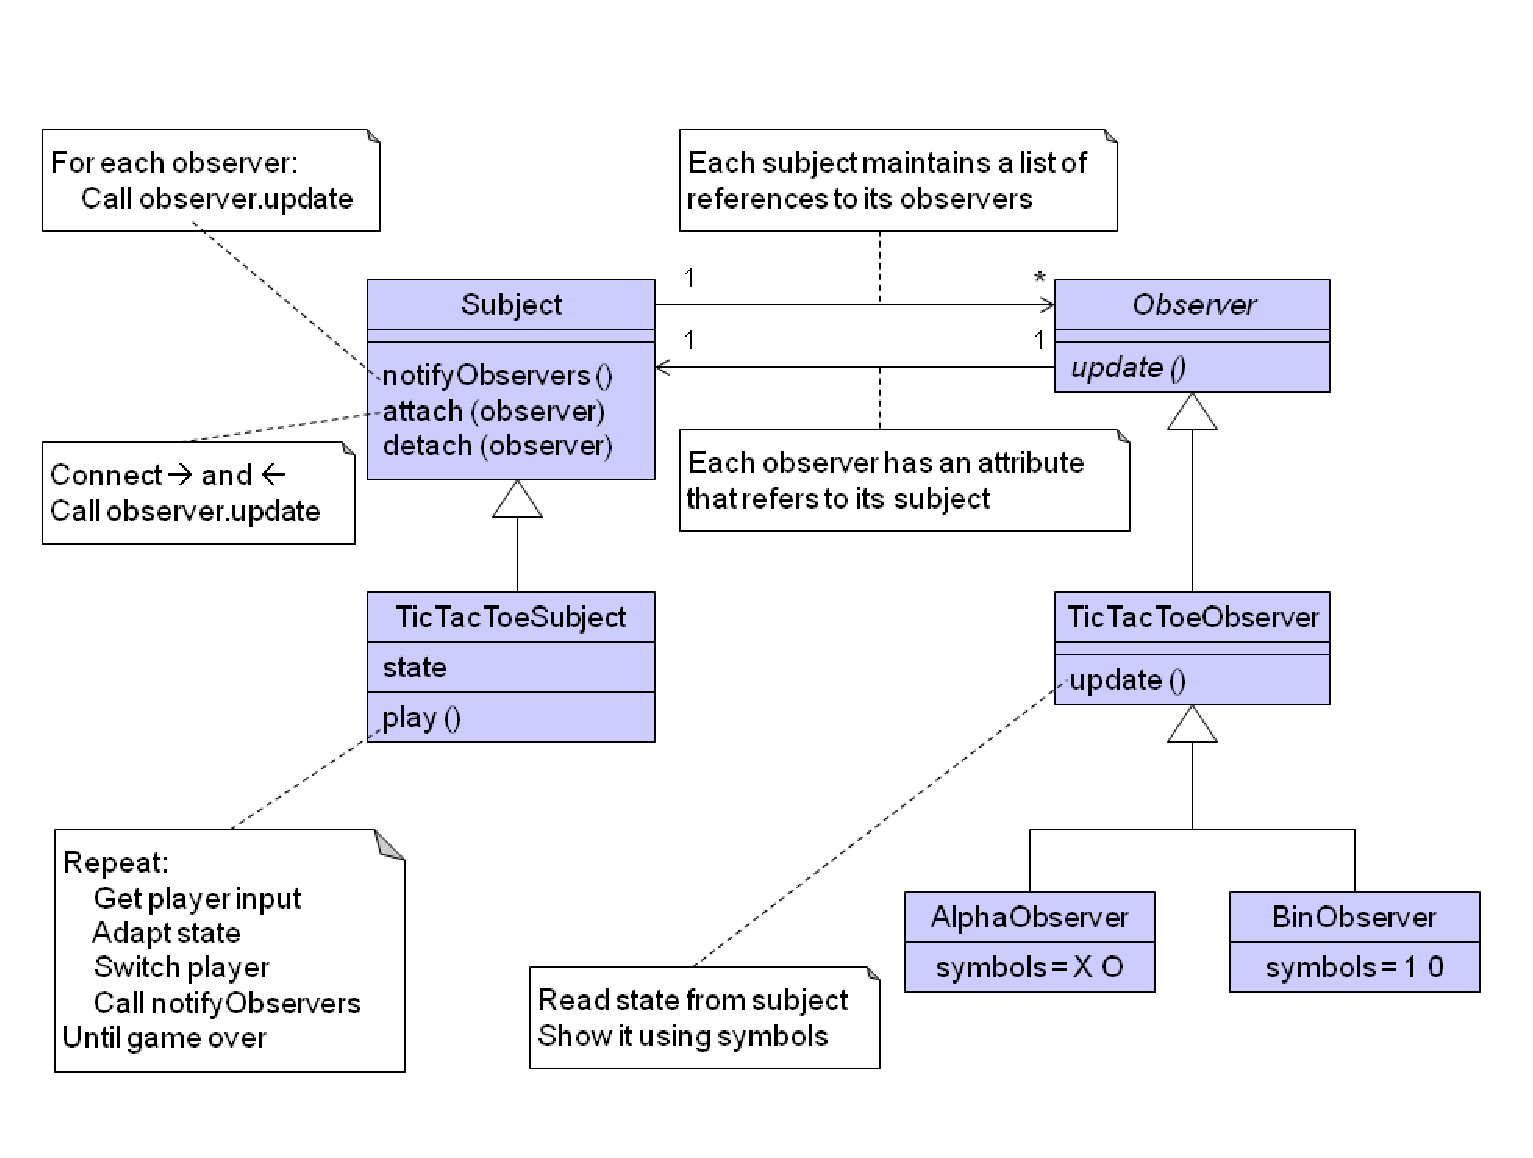
\includegraphics[width=15cm]{imag/patterns/observer}
\caption{Tic Tac Toe Observer example}
\end{figure}


\emph{TicTacToeSubject} contains the game logic, altering the game
\emph{state} with each move\emph{. TicTacToeSubject} is a specialization
of the \emph{Subject} class, embodies one halve of the Observer pattern.
Subjects are able to \emph{attach} observers to themselves by placing
them into an \emph{observers} list and storing a back reference in
\emph{subject} attribute of the \emph{observer} as well. They then
can notify their observers of any changes by means of their \emph{notifyObservers}
method, that will call the \emph{update} method on each observer.

Class \emph{Observer} embodies the other halve of the Observer pattern.
The \emph{Observer} class has an \emph{update} method. It is just
there to define the interface, not to do anything useful. Such a method
is called abstract, and its name is italicized in the diagram. Having
at least one abstract method makes the whole \emph{Observer }class
abstract, since no fully functional objects can be instantiated from
it. So the name of the \emph{Observer }class is italicized as well.

Class \emph{TicTacToeObserver} inherits from \emph{Observer}. Its
\emph{update }method reads the state from the \emph{TicTacToeSubject}
and displays it. It isn't called directly on a \emph{TicTacToeObserver},
but on an \emph{AlphaObserver} or a \emph{BinObserver} that inherit
this method, so it uses the\emph{ symbols} of one of these descendant
classes.  

\subsection{Example code}

\shadowbox{\begin{minipage}[t]{1\columnwidth}%
TIP: The class diagram showed in broad lines how the Tic Tac Toe example
works. If you use diagrams like that, keep them simple. The right
place for details is properly commented source code. Avoid complicated
diagramming tools, that subvert freedom of expression by enforcing
all kinds of strickt rules. Diagrams are only there to help imagination
a bit.%
\end{minipage}}

Having understood the class diagram, you're now ready for the real
thing: Use the force, read the source!

\lstinputlisting[caption={patterns/observer.py},label={lst:patterns/observer}]{prog/patterns/observer.py}

\section{The Adapter pattern}
\subsection{Example situation}

This example is about a tiny part of a control for an Automated Stacking
Crane or ASC. ASC's store and retrieve containers that are kept in
stock by even thousands in the so called stacking area of a container
terminal. All ASC's together are controlled by the so called Movement
Planner. The task of the Movement Planner to plan for efficient storage
and retrieval of containers, e.g. keeping containers that have to
leave first on top of the stacks or or put interchangeable containers
on top of each other. The Movement Planner works with an elementary
displacement from A to B called a \emph{move}. The cranes, however,
works with so called \emph{get} and \emph{put} orders. To \emph{move}
a container from A to B it has to first receive a \emph{get} order,
to pick it up at A, and then a \emph{put} order to put it down at
B. So there's a mismatch between how the Movement Planner requests
a displacement (\emph{move} interface) and how the ASC expects to
receive it (\emph{get} and \emph{put} interface). Since there's a
mismatch between these two interfaces, what's needed is an adaptor.

\subsection{Solution principle}

Adaptors come in two kinds, the first one being the Object Adapter:

\begin{figure}[H]
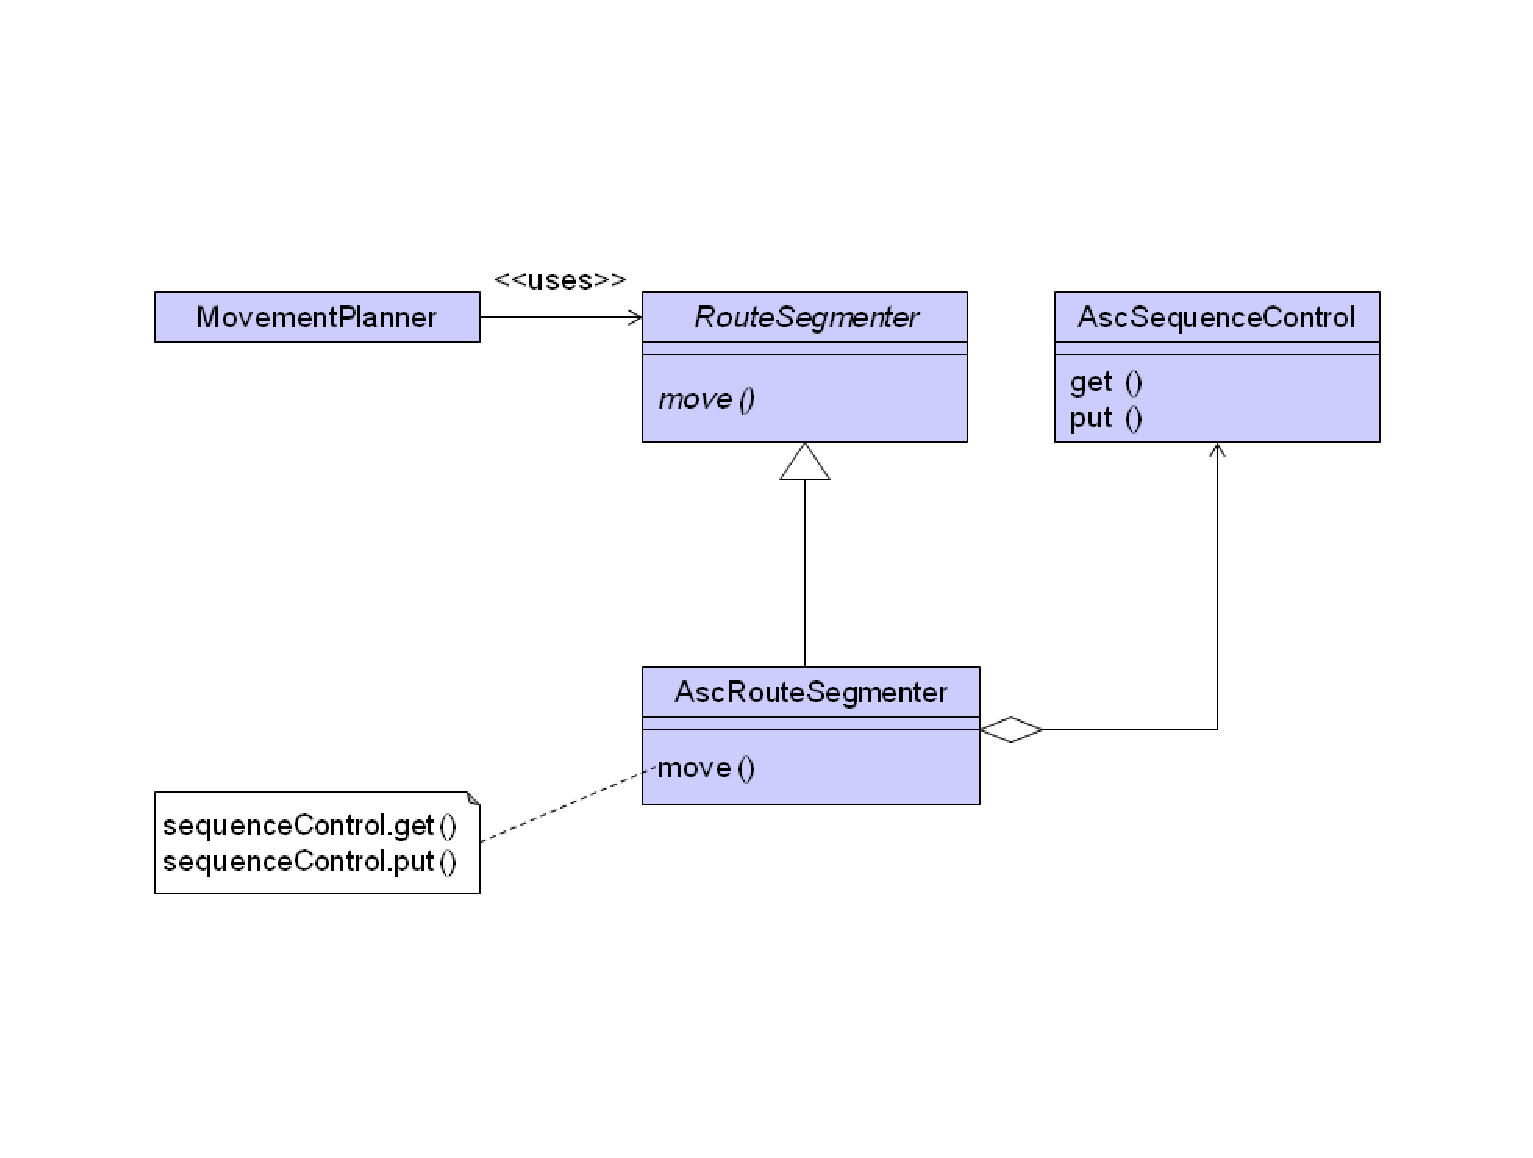
\includegraphics[width=15cm]{imag/patterns/objectAdapter}
\caption{ASC Object Adapter example}
\end{figure}

The interface of class \emph{RouteSegmenter }consists of the \emph{move}
method, as required by the \emph{MovementPlanner}. The \emph{AscSequenceControl}
has an interface consisting of the \emph{get} and \emph{put} methods.
Class \emph{AscRouteSegmenter} inherits its interface from \emph{RouteSegmenter}.
It contains an attribute of type\emph{ AscSequenceControl} and it
implements its\emph{ move }interface method by calling \emph{get}
and \emph{put} upon this attribute. The \emph{get }and \emph{put }methods
themselves are not added to the interface. Moreover it is possible
for an \emph{AscRouteSegmenter} to contain multiple instances of \emph{AscSequenceControl}.

The other kind of adapter is the Class Adapter:

\begin{figure}[H]
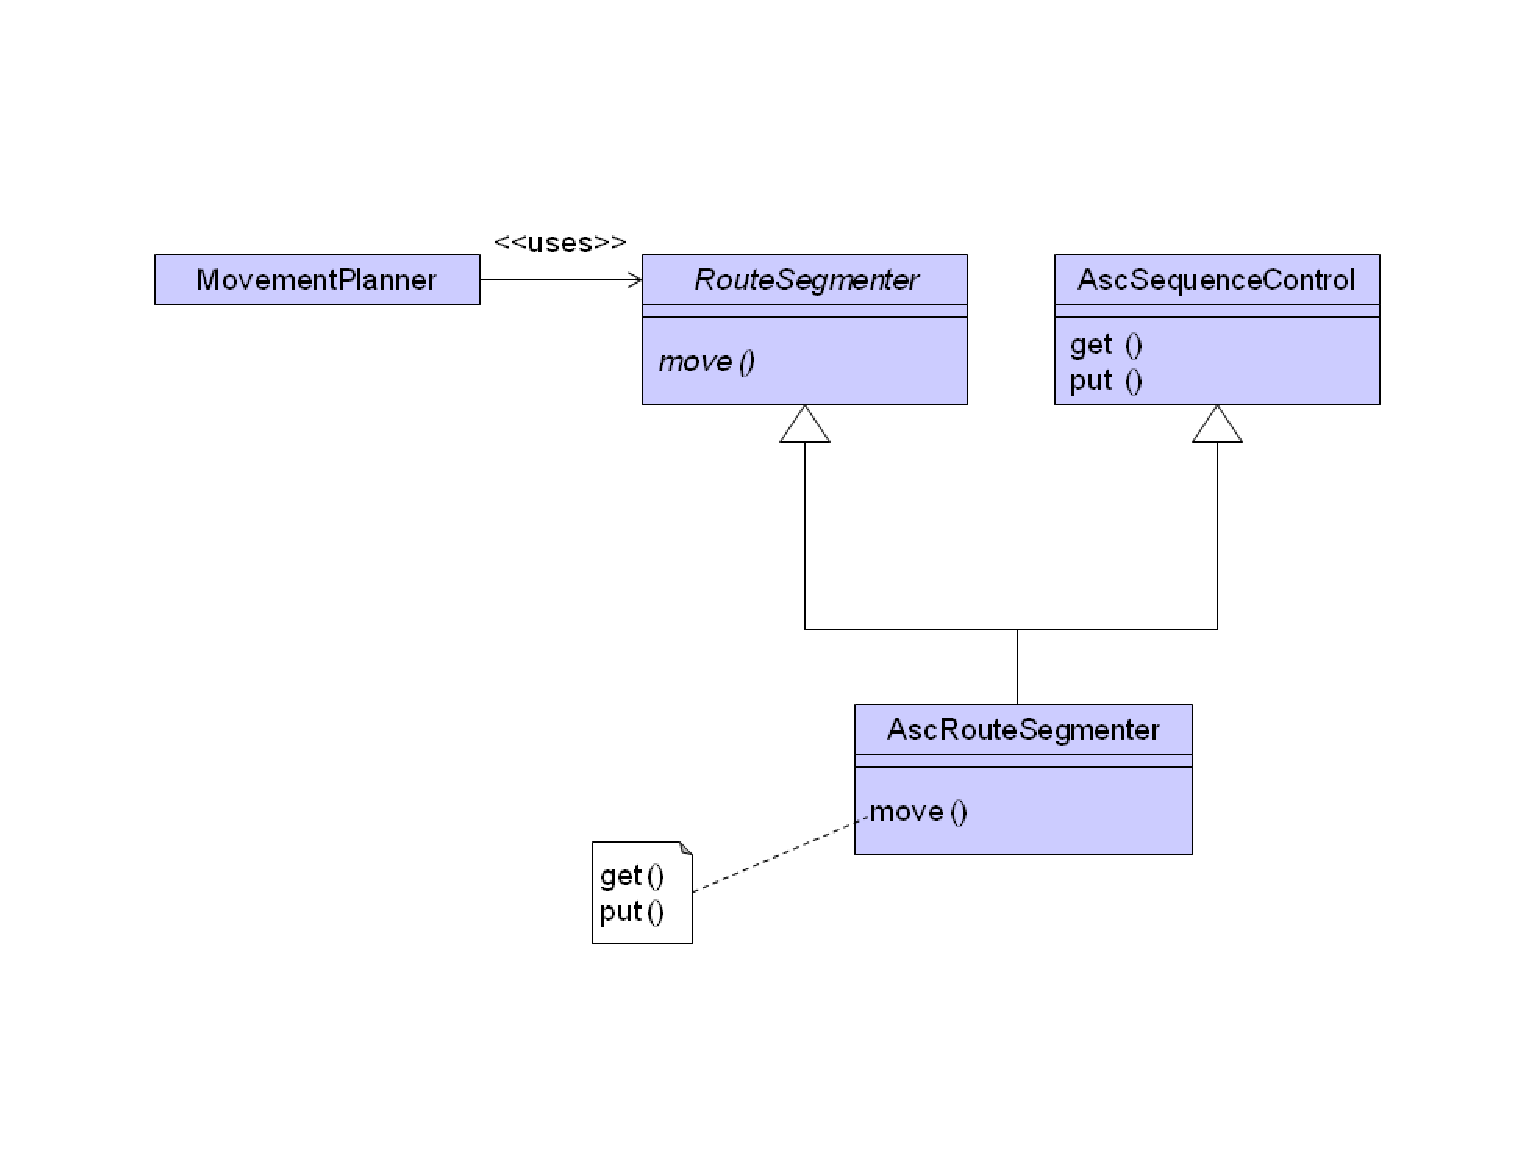
\includegraphics[width=15cm]{imag/patterns/classAdapter}
\caption{ASC Class Adaper example}
\end{figure}

Class \emph{AscRouteSegmenter }now inherits from both the \emph{RouteSegmenter
}interface class and from the \emph{AscSequenceControl }class that
contains the implementations of \emph{get} and \emph{put}. Interface
method \emph{move }now calls these two inherited methods, not via
an attribute but directly. Note that the \emph{AscRouteSegmenter}
does \noun{not contain} an \emph{AscSequenceControl} in that case,
it \noun{is} an \emph{AscSequenceControl}. This means that its interface
contains \emph{move} as well as \emph{get }and \emph{put}. And there
can't be multiple instances of \emph{AscSequenceControl} embedded
in one \emph{AscRouteSegmenter}.

\subsection{Example code}

The code of the object adaptor version is:

\lstinputlisting[caption={patterns/objectAdapter.py},label={lst:patterns/objectAdapter}]{prog/patterns/objectAdapter.py}

The code of the Class Adapter is slightly more compact:

\lstinputlisting[caption={patterns/classAdapter.py},label={lst:patterns/classAdapter}]{prog/patterns/classAdapter.py}

Nevertheless, in most cases use of the Object Adaptor is to be preferred
for two reasons:
\begin{enumerate}
\item In general, it is desirable if interfaces are stable and thin. Stable
means that they do not have to be changed with every minor change
of the design. Standardization only reduces costs if you can rely
on standards not constantly changing. Thin means that there are not
too many methods or attributes that are part of the interface. Having
a lot of methods or attributes in the interface of a class entails
that some code elsewhere in the program may be dependent upon the
presence of all those methods or attributes. In our class adapter
example the \emph{get }and\emph{ put }of \emph{AscSequenceControl
}are inherited and become part of the interface of \emph{AscRouteSegmenter}.
As a consequence of this, the amount of work involved in changing
the interface of \emph{AscSequenceControl }(\emph{get }and \emph{put})
could be unnecessarly high, since not only code that uses \emph{AscSequenceControl
}directly but also code that uses \emph{AscRouteSegmenter} would have
to be changed.
\item The possibility to have multiple instances of \emph{AscSequenceControl}
embedded in one \emph{AscRouteSegmenter} contributes to the flexibility
of the design.
\end{enumerate}
\shadowbox{\begin{minipage}[t]{1\columnwidth}%
BACKGROUND: A common misunderstanding is that encapsulation is about
hiding attribute data by only accessing them via methods that store
or retrieve them. But the main benefit of encapsulation is more general:\medskip{}

\noun{\hspace{1cm}Encapsulation is about hiding}\emph{\noun{ }}\noun{design
decisions}\emph{\noun{ }}\noun{rather than about data hiding.\medskip{}
}

Hiding a design decision means that changing this decision has only
local impact. This contributes to the flexibility of the design, since
the costs of change are limited. Changing an attribute indeed boils
down to changing a design decision, but so does changing a method.
So striving for thin interfaces is not only about hiding attributes
but also about hiding methods. Hiding data may have extra benefits,
apart from hiding design decissions. That's what \secref{thePropertyPattern}
is about.%
\end{minipage}}

\section{The Property pattern\label{sec:thePropertyPattern}}
\subsection{Example situation}

Suppose we have a \emph{Circle }class which has the attributes \emph{radius},
\emph{perimeter }and \emph{area }in its interface. It seems that the
'thin interfaces' principle would indicate that e.g. only the \emph{radius
}should be present in the interface. But since any real world circle
also has a perimeter and an area, no generality is sacrificed by adding
them to the interface. And by adding them, code that uses \emph{Circle}
could directly use \emph{perimeter }and \emph{area} in addition to
\emph{radius}. Storing them as separate attributes would unfortunately
mean that they have to be kept in sync explicitly. As an alternative
to having the attributes \emph{perimeter} and \emph{area}, we could
use methods \emph{getPerimeter} and \emph{getArea} to compute those
values on the fly. And we could also add methods \emph{setPerimeter}
and \emph{setArea}, to set the \emph{radius }via them. Doing so would
would result in a \emph{Circle} interface consisting of \emph{radius},
\emph{getPerimeter},\emph{ setPerimeter},\emph{ getArea }and\emph{
setArea.} This unnecesarily exposes the design decision that the radius
is actually stored, while the perimeter and the area are computed
on the fly. Suppose that after a while, the area of the circle would
turn out te be used much more frequent than the radius. Then it would
become more attractive to store the area and compute the radius and
the perimeter from that. This would lead to a changed interface of
\emph{Circle, }consisting of \emph{getRadius}, \emph{setRadius}, \emph{getPerimeter},
\emph{setPerimeter }and \emph{area}, so all the code using \emph{Circle}
would have to be adapted. We'd like to avoid that expensive overall
changes like that. How to proceed?

\subsection{Solution principle}

One way to go, is to add a getter and setter to the attribute itself
as well, right from the start. The interface of \emph{Circle} would
then become: \emph{getRadius}, \emph{setRadius}, \emph{getPerimeter},
\emph{setPerimeter getArea}, \emph{setArea. }The decision which value
is actually stored and which other two are computed from it is then
hidden. This means that we're free to switch from storing \emph{\_radius}
to storing \emph{\_perimeter} or \emph{\_area }at any time. Remember
that prepending \emph{\_} to an attribute or method means that it
does not belong to the interface. That is important here, because
if people started to directly access \emph{\_radius}, storing \emph{\_area}
instead would still break their code, requiring extra work. 

\shadowbox{\begin{minipage}[t]{1\columnwidth}%
BACKGROUND: Some of the practical thinking behind Python is revealed
by the fact that refraining from direct use of private attributes
or methods (the ones that start with a single \_) is left to free
will.\medskip{}

There may be very good reasons to directly use a private attribute
or method afterall, just like there may be very good reasons to break
into your own car if you locked in the keys. Computer programs live
in the real world, not in an ideal one.%
\end{minipage}}

An attribute that is meant to be only accessed via a getter or a setter
is called a property. Python supports properties in an elegant way.
Rather than having the bulky \emph{getRadius}, \emph{setRadius}, \emph{getPerimeter},
\emph{setPerimeter, getArea}, \emph{setArea} interface, that requires
the design decision to use a propery to be taken up front, since all
external code depends upon this interface, it allows you to maintain
the original \emph{radius}, \emph{perimeter}, \emph{area} interface
while still using properties.

Without this facility, one might indeed be inclined to use getters
and setters for each attribute, just to be prepared for the unknown.
With it, one can start out with simple attributes and change them
to properties whenever needed, without impacting the rest of the design.
It is important to make a clear distinction here: Accessing attributes
via getters and setters is called the Property pattern. The fact that
Python has transparent way to do so is a bonus, but stricktly spoken
not part of the pattern. Since you're learning Python here, we'll
shamelessly benefit of that bonus in the example code.

\subsection{Example code}

In the first example, the only thing actually stored in an object
of class \emph{Circle }is the private \emph{\_radius} attribute. All
access to this attribute, including access via the methods of \emph{Circle}
itself, is via the associated public \emph{radius} property. Note
that the getters and setters start with an \emph{\_, }since they are
never to be called directly by code outside the class. The interface
of \emph{Circle} consists of the \emph{radius}, \emph{perimeter }and\emph{
area }properties. This interface hides the design decision on what
is actually stored.

\lstinputlisting[caption={patterns/propertyRadius.py},label={lst:patterns/propertyRadius}]{prog/patterns/propertyRadius.py}

In the second example, not the \emph{\_radius}, but the \emph{\_area}
is stored in a private attribute. The interface of \emph{Circle} still
consists of the \emph{radius}, \emph{perimeter }and\emph{ area }properties.
Since the interface did not change at all, all code using \emph{Circle
}doesn't have to change with respect to the previous example. This
is a direct benefit from \emph{Circle} having a stable interface,
that doesn't change when \emph{\_area} instead of \emph{\_radius}
is stored. \lstinputlisting[caption={patterns/propertyArea.py},label={lst:patterns/propertyArea}]{prog/patterns/propertyArea.py}

\shadowbox{\begin{minipage}[t]{1\columnwidth}%
TIP: The fact that the member functions of \emph{Circle }also use
\emph{radius}, \emph{perimeter }and\emph{ area}, rather than calling
getters and setters or accessing the private attribute directly, further
limits the impact of design changes. One might argue that accessing
the underlying attribute (\emph{\_radius} or \emph{\_area}) directly
may result in faster code. This type of so called ``peephole optimization''
should be avoided if possible, since it violates the DRY principle.
This makes design changes harder, including the optimizations that
\noun{really} matter. As a general rule:

\medskip{}
\noun{\hspace{1cm}Don't start optimizing too early, first give priority
to a clear and regular design.}

\medskip{}
This is not an invitation to be wasteful, but to avoid being ``penny
wise and pound foolish''. If you've defined a standard interface
for a class, use it, also in the class itself. O, and yes indeed,
there are exceptions to any rule, this one is no exception.%
\end{minipage}}

\section{{*}EXTRA{*} The Call Chaining pattern}

\shadowbox{\begin{minipage}[t]{1\columnwidth}%
TIP: While the call chaining pattern itself isn't too difficult, the
example given here is complicated. It uses a lot of special Python
facilities and some clever tricks. Depending on your skills you may:
\begin{enumerate}
\item Skip this pattern altogether. Not much is lost if you do.
\item Superficially skim through \subref{Example-situation} , study the
small code blocks in \subref{Solution-principle} thoroughly, but
skip \subref{Example-code} completely.
\item Wrestle through \subref{Example-code} as well.\end{enumerate}
%
\end{minipage}}

\subsection{Example situation\label{sub:Example-situation}}

The first time I encountered the Call Chaining pattern was in IBM's
Visual Age library in 1980. I started to use it myself every now and
then. Later on it became part of the Microsoft's LINQ. LINQ makes
it possible to select data from a collections of object in a clever
way, inspired by SQL. SQL (pronunciation: sequel) or Structured Query
Language is a special purpose language to query and update data in
a so called relational database, a very popular way to store data
into tables on disk.

An example of a SQL statement is:

\begin{lstlisting}
SELECT name, address
FROM customers
WHERE profit > 10,000,000
\end{lstlisting}

Spent a few minutes reading bout SQL e.g. in Wikipedia. Don't dive
to deeply, most of it will be intuitively clear. While SQL is a language
in its own right, often the need arises to have SQL statements as
part of e.g. a Python program. One way to do that is just to embed
them as multi line strings (Google for Python and 'multiline strings'):

\begin{lstlisting}
query = '''
	SELECT name, address
	FROM customers
	WHERE profit > 10,000,000
'''

result = database.execute (query)
\end{lstlisting}

In this code fragment \emph{query }is a string variable containing
a piece of SQL. Python doesn't have any idea about the meaning of
this piece of SQL, but just passes the string as parameter to method
\emph{execute} of a Python object of class \emph{database}. That object
just forwards the contents of the SQL string to a special purpose
program called the RDBMS (Relational Database Management System).
The RDBMS queries the database and returns the selected data to the
\emph{execute} function that in turn returns it to \emph{result}.
This can be done, since the RDBMS can be controlled from C/C++ and
Python in turn can communicate with C/C++ code, a.o by using something
called Cython. The details are not relevant at this point and, on
top of that, rather boring. An RDBMS that Python plays nice with is
SQLite, but all the others will do as well.

Another way to use SQL from Python is to have special functions in
Python like \emph{SELECT}, \emph{FROM} and \emph{WHERE}, to do the
querying. The nice thing about this approach is that these functions
may be programmed in such a way that they query Python lists rather
than a real SQL database. This example gives you an idea of how that
might be done in principle. The main thing you can learn from it,
is that there's no mystery involved in SQL, or anything else that
has to do with computer programming for that matter. So, we are not
going to connect to any RDBMS. Rather we'll select data from Python
lists. But an interface to an RDBMS could be added. This is exactly
what Microsoft did with their LINQ tool. As with LINQ, the language
we'll use (or rather, make) is not SQL, but something that looks a
lot like it, allowing constructions like:

\begin{lstlisting}
result = (
	FROM (animals) .
	WHERE (lambda r: r.species == 'human' and r.age > 10) .
	SELECT (lambda r: (r.gender, r.name, r.age)) .
	ORDER_BY (lambda r: (r.name, r.age | DESC))
)
\end{lstlisting}

Here the SQL query is not a 'dead' string that doesn't mean anything
to Python, it is an alive and kicking chain of Python function calls,
each of the functions able to do something useful as part of the query.
The secret of this code is in the dots at the end of the lines. It's
these dots that give away the Call Chaining pattern.

\subsection{Solution principle\label{sub:Solution-principle}}

The solution principle of call chaining is that each call to a function
or method returns an object. From this object in turn a method can
be called, which returns another object, of which a method can be
called, and so on. In the above piece of code the \emph{FROM} function
returns an object of class \emph{Table}. Class \emph{Table} has a
method \emph{WHERE}, that returns second object, holding a selection
of the first \emph{Table} object. This second object is also of class
\emph{Table}. Class \emph{Table} also has a method \emph{SELECT}.
This method again returns a \emph{Table} instance. Class \emph{Table}
also has a method \emph{ORDER\_BY}, which is called in the end, returning
a string with a sorted version of the contents of the \emph{Table}.

The dots were crucial because they provide the glue between the lines
of SQL like code. If \emph{FROM (animals)} returns an object, then
F\emph{ROM (animals) .WHERE (...)} is just a method call upon that
object. It is the normal dot notation for calling methods that we've
used everywhere. So the essence of the pattern is that rather than
writing:

\begin{lstlisting}
object1 = functionA ()
object2 = object1.methodB ()
object3 = object2.methodC ()
object4 = object3.methodD ()
result = object4.methodE ()
\end{lstlisting}

one writes:

\begin{lstlisting}
result = (
	functionA () .
	methodA () .
	methodB () .
	methodC () .
	methodD ()
)
\end{lstlisting}

Each method call relies upon the result of the previous call. It is
as if the object returned by functionA is handed through a sequence
of transformation functions. With database querying each transformation
acts as a filter narrowing down the query. But call chaining like
this can also be used to e.g. transform graphical objects:

\begin{lstlisting}
render (
	getCube () .
	stretchX (3) .
	stretchY (4) .
	rotateX (math.pi / 2) .
	material (shiny) .
	light (green)
)
\end{lstlisting}

The final stretched, rotated , illuminated object is returned to the
\emph{render} function, that puts it on the screen.

\subsection{Example code\label{sub:Example-code}}

The example code uses a small selection of the many under-the-hood
features that make Python such a power tool. They will be explained
in a second, heavily commented, version of the source code. But first
traverse the bare code criss-cross with a machete and see what you
pick up from it without any explanation. Maybe the end is the best
place to start, since that's where everything comes together. Don't
strive for complete understanding, just get some intuitive sense of
what this code roughly does. If some fragments are too hard, skip
them. If this leads you to skipping everything, that's completely
OK.

\lstinputlisting[caption={patterns/callChaining.py},label={lst:patterns/callChaining}]{prog/patterns/callChaining.py}

Next thing to look at is an abundantly commented version of the same
code. Using comments like this is called Literate Programming. Give
it another go, carefully reading the comments. Be prepared to do some
detective work.

\lstinputlisting[caption={patterns/callChainingLiterate.py},label={lst:patterns/callChainingLiterate}]{prog/patterns/callChainingLiterate.py}

--//--

\end{document}
